\documentclass[../main.tex]{subfiles}
\begin{document}
    

\section{Matplottoy}

We build on the existing Matplotlib architecture \cite{hunterMatplotlib2DGraphics2007} so that we can initially focus on the data to graphic transformations and rely on Matplotlib for the other graphical elements of the visualization and the rendering. We first introduce an implementation of scatter, line, and bar charts because they map to the fundemental marks of point, line, and area. We then introduce aggregated bar charts to show how to build more complex graphics.  

Because we do not expect the user to specify every visual parameter, we define a class of required visual variables that are intrinsic to S. %%need to revise for formality but
What I mean here is that you cannot construct the mark w/o this - position for scatter \& line, values for heatmap. 

\subsection{Scatter}
 A scatter plot \cite{friendlyBriefHistoryData2006a,tukeyExploratoryDataAnalysis1977} is a chart type for plotting discrete values against each other. Minimally a scatter plot requires and x or y position, but the other variables in our dataset can be mapped to visual aspects of the scatter graphical mark. 
\begin{figure}[H]
    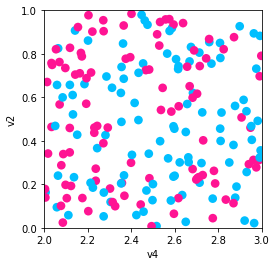
\includegraphics[width=\textwidth]{figures/code/scatter_0.png}
    \label{fig:scatter}
\end{figure}

For the scatter plot in figure~\ref{fig:scatter}, we define $Q$ as 
 \begin{equation}
    Q(\mu_{xpos}, \mu_{ypos}, \mu_{facecolor}, \mu_{s})
    \label{eq:scatter}
 \end{equation}

which we implement building on the \texttt{matplotlib.collections} API:

\begin{minted}{python}
    class Point(mcollections.Collection):
        # this is the visual fiber 
        required = {'x', 'y'}
        optional = {'facecolors', 's'} 
        def __init__(self, data, transforms, *args, **kwargs):
            # check that the constraints on Q can be met  
        def draw(self, renderer, *args, **kwargs):
            # assemble the glyph
            super().draw(renderer, *args, **kwargs)
    \end{minted}
    
(subject to change). Unlike equation~\ref{eq:scatter}, we pass also pass a reference to the data so that getting the data can be fully curried until absolutely necessary. The \texttt{*args} and \texttt{**kwargs} are artifacts of using Matplotlib as a base. We pass in the $\mu$ as the dictionary "transforms" mostly for readability, which is also why we define the visual fiber as class attributes.

Inside the \texttt{__init__} constructor, is a check if there is a valid mapping between $S$ and $K$.  Line 7-8 check if the user has passed in the required $\mu$ and whether the $\nu$ functions are valid for the input data.

\begin{minted}[lineno]{python}
def __init__(self, data, transforms, *args, **kwargs):
    super().__init__(*args, **kwargs)
    # check that the data you're trying to transform 
    # has a way to provide vertex data  
    assert 'vertex' in data.FB.K['tables']
    # check that you've given the required parameters
    utils.check_constraints(Point, transforms.keys())
    utils.validate_transforms(data.FB.F, transforms)

    self.data = data
    self.transforms = transforms
\end{minted}

Lines 9-10 attach the data and transforms to the $Point$ object as a concession to the Matplotlib architecture that seperates drawing from creation. In \texttt{draw}, the attributes of the graphic are set to the different sections of the visual fiber bundle. 

\begin{minted}[lineno]{python}
def draw(self, renderer, *args, **kwargs):
    view = self.data.view('vertex') #resolve to size
    
    # \nu(\tau)
    visual = utils.convert_transforms(view, self.transforms)
        
    # assembles taus to generate idiom
    visual['s'] = itertools.repeat(visual.get('s', 0.05))
    visual['facecolors'] = visual.get('facecolors', "C0")
    #switch out to a marker 
    self._paths = [mpath.Path.circle(center=(x,y), radius=s)  
                    for (x, y, s) 
                    in zip(visual['x'],visual['y'], visual['s'])] 
    
    self.set_facecolors(visual['facecolors'])
    super().draw(renderer, *args, **kwargs)
\end{minted}
Line 1 pulls back into the data bundle and returns $\tau = \{\tau_0, \ldots, tau_{n}\}$. Line 3 applies the transforms $\nu$ to $\tau$ to build the visual bundle $V$.  Line 8 sets the abstract segment marks with the visual characteristics. Line 10 passes this information to the renderer, acting like a $rho$. 

The visual fiber bundle is specified as a dictionary $\{\mbox{parameter}: (\mbox{variable}, \nu), \mbox{parameter}:\mbox{value}\}$ 
\begin{minted}[lineno]{python}

transforms = {'y': ('v2', position.Identity()),       
              'x': ('v4', position.Identity()),
              'facecolors': ('v3', color.Categorical( {'true':'deeppink', 'false':'deepskyblue'})), 
              's':.01}
\end{minted}

where the $\nu$ functions are represented as classes so that parameters can be curried. For example, \texttt{color.Categorical} is a whole set of $\nu$ functions explicitly tuned to specific categorical mappings. A pure functional approach would mean the user would have to write new functions

\begin{minted}[lineno]{python}
def color_true_deepink_false_deepink(value):
    return {'true':'deeppink', 'false':'deepskyblue'}[value]

\end{minted}

for every categorical colormapping, which would be somewhat untenable. An alternative approach could be to partially curry:

\begin{minted}[lineno]{python}
     'facecolors': ('v3', (color.categorical, {'true':'deeppink', 'false':'deepskyblue'}))
\end{minted}

but that doesn't allow for as easy reuse? (I should probably actually just switch to this form) The \textt{color.categorical} function is implemented as 
\begin{minted}[lineno]{python}
class Categorical:
    def __init__(self, mapping):
        """goal of init is to store parameters that would otherwise be
        curried higher level function"""
        assert(mcolors.is_color_like(color) for color in mapping.values())
        self._mapping = mapping

    def convert(self, value):
        values = np.atleast_1d(np.array(value, dtype=object))
        return [mcolors.to_rgba(self._mapping[v]) for v in values]

    def validate(self, mtype):
        return mtype in ['nominal']
\end{minted}

where the \texttt{convert} function converts the input value to the internal normalized form Matplotlib expects. The `\texttt{validate}' function checks which monoid actions the transform supports; optimally this method should be replaced by functions that check the properties, for example a \texttt{is_ordinal} method that checks that monotonicity is preserved. 

#does the data even matter?

\end{document}